\chapter{Desenvolvimento}
\label{chap:Chapter5}
Após a idealização do modelo é conveniente a sua aplicação prática. Nesse sentido, este capítulo aborda o processo de desenvolvimento do protótipo, um \textit{chatbot} que recebeu o nome \textit{Proto}, construído com base no modelo proposto, usando os serviços cognitivos da Microsoft disponíveis na \textit{cloud}. No decorrer do capítulo enuncia-se o processo de implementação do protótipo, fazendo referência à transposição do modelo para a prática, da configuração necessária, nomeadamente das bases de conhecimento, e detalhes relevantes da desenvolvimento desta prova de conceito.

%%%%%%%%%%%%%%%%%%%%%%%%%%%%%%%%%
%           SECTION
%%%%%%%%%%%%%%%%%%%%%%%%%%%%%%%%%
\section{Especificação}
\label{sec:chap05_specification}
Dado o modelo proposto (ver Capítulo~\ref{chap:Chapter4}), é crucial a sua transposição para a realidade dum \textit{chatbot}. Como referido anteriormente, este foi desenvolvido usando os serviços cognitivos da Microsoft, sendo então pertinente a introduzir alguns conceitos gerais e a arquitetura que foi especificada.

\subsection{Visão Geral}
Um \textit{chatbot} é um tipo de \gls{iln} que providencia uma experiência rica ao utilizador, dando-lhe a sensação que está a comunicar com outro ser humano~\parencite[Concepts]{microsoft_bot_documentation}.
Conforme descrito em~\textcite[Principles of bot design]{microsoft_bot_documentation}, um \textit{chatbot}, tal como qualquer outra interface, para além de garantir uma ótima experiência de utilização, deve também seguir quatro orientações:

\begin{enumerate}
    \item 
    {
        Resolução do problema do utilizador com o mínimo de etapas possível;
    }
    \item
    {
        Apresentação de uma solução de forma mais fácil e rápida do que as suas alternativas;
    }
    \item 
    {
        Disponibilidade em diferentes dispositivos e plataformas;
    }
    \item 
    {
        Fácil acessibilidade, garantindo que o utilizador sabe exatemente o que fazer.
    }
\end{enumerate}

Neste quadro, o protótipo deve ter a capacidade de conversação aliada à responsabilidade de transmitir a informação pretendida, quando requisitada pelo utilizador. Para este efeito, os serviços cognitivos da Microsoft (Azure Cognitive Services) disponibiliza dois serviços~\parencite{microsoft_luis_use_nl_processing_service}: o Microsoft LUIS e QnA Maker (ver Figura~\ref{fig:prototype_overview}).
%
\begin{figure}
    \centering
    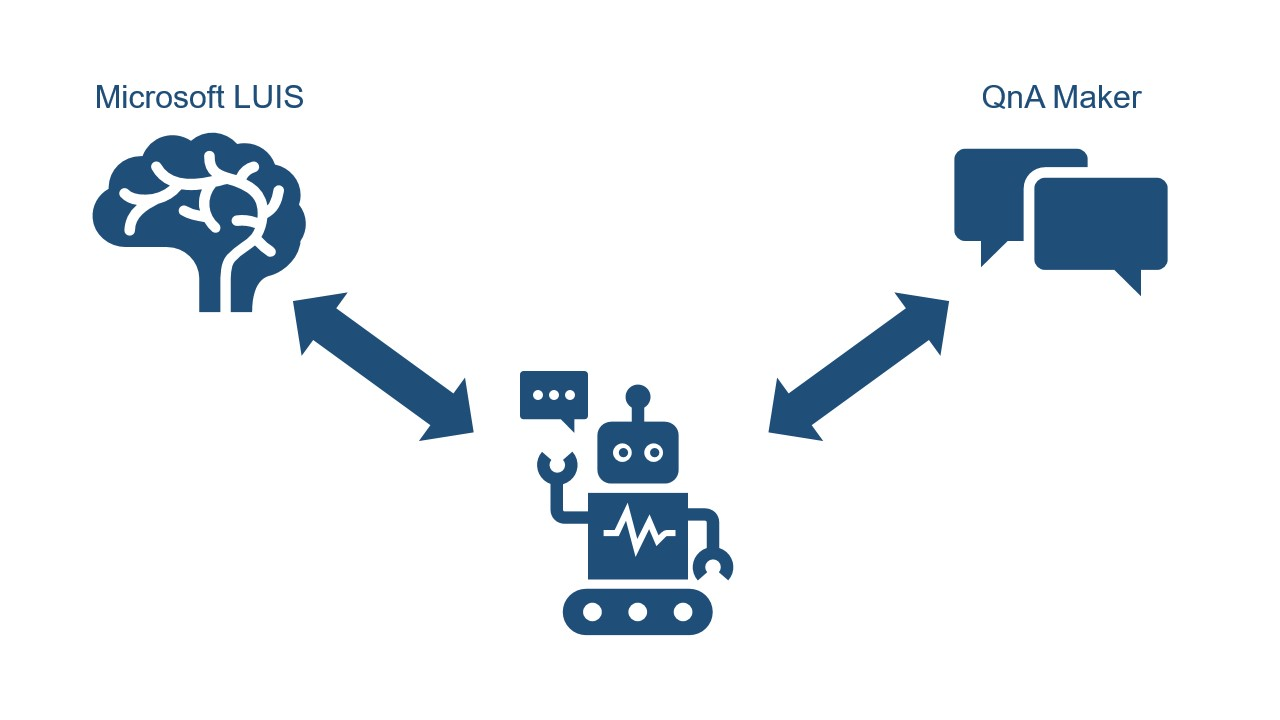
\includegraphics[width=.8\textwidth]{ch05/assets/prototype-overview.jpg}
    \caption{Vista geral da interação entre o \textit{chatbot} e os serviços disponibilizados}
    \label{fig:prototype_overview}
\end{figure}

O Microsoft LUIS mantém a base de conhecimento referente às intenções e entidades, tendo a capacidade de compreensão de linguagem natural. Por outro lado, o QnA Maker age como um dicionário, no qual contém respostas estáticas face a perguntas pré-definidas que não tenham uma intenção específica. Ao \textit{chatbot} cabe a responsabilidade de orquestrar o processo de conversação, ficando encarregue de executar as ações vinculadas à intenção identificada pelo Microsoft LUIS ou \inquotes{conversar} com o utilizador, quando nenhuma intenção é identificada, obtendo respostas-padrão contidas QnA Maker.

Para trabalhar com estes serviços, a Microsoft disponibiliza um conjunto de ferramentas \textit{open source}, Bot Framework Tools\footnote{Disponível em \url{https://github.com/microsoft/botframework\#bot-framework-tools}.}, que ajudam no desenvolvimento e suporte de soluções. No caso do Microsoft LUIS, é também facultada uma \gls{api} na \textit{Web}.

\subsection{Arquitetura}
Tendo em conta a visão geral apresentada e o modelo proposto, a Figura~\ref{fig:prototype_architecture} mostra a arquitetura definida para o protótipo, ao qual se deu o nome de \textit{Proto}. A seguir, faz-se uma descrição de cada componente e de que forma se enquadra na arquitetura do modelo previamente especificado.
%
\begin{figure}[!ht]
    \centering
    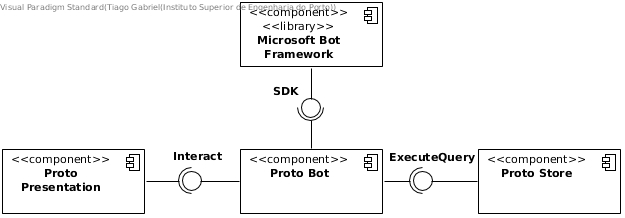
\includegraphics[width=.75\textwidth]{ch05/assets/prototype-architecture.jpg}
    \caption{Arquitetura do protótipo, seguindo o modelo proposto}
    \label{fig:prototype_architecture}
\end{figure}
%
\begin{itemize}
    \item
    {
        \textit{Proto Presentation} -- responsável pela interação com o utilizador. No modelo corresponde ao componente \textit{NL Presentation};
    }
    \item
    {
        \textit{Proto Bot} -- o \textit{chatbot} propriamente dito. Tal como o seu análogo no modelo, o \textit{QA Service}, conhece as partes envolvidas no processo, portanto orquestra-o;
    }
    \item
    {
        \textit{Microsoft Bot Framework} -- a biblioteca que dispõe o acesso às bases de conhecimento, possibilitando o reconhecimento das entidades e a aquisição de respostas estáticas. Por outras palavras, permite o acesso ao Microsoft LUIS e ao QnA Maker. Equivale ao \textit{Comprehension Service} presente no modelo proposto;
    }
    % \item
    % {
    %     \textit{Proto Feedback Store} -- representa a parte da base de conhecimento de domínio (\textit{NL Knowledge Base}) que guarda o \textit{feedback} obtido. Para efeitos de protótipo, é aceitável que se mantenha como um componente separado, visto que não é possível guardar esta informação nas bases de conhecimento mantidas na \textit{cloud};
    % }
    \item
    {
        \textit{Proto Store} -- simula o armazém de dados de negócio. Análogo do componente \textit{Production Store}.
    }
\end{itemize}

%%%%%%%%%%%%%%%%%%%%%%%%%%%%%%%%%
%           SECTION
%%%%%%%%%%%%%%%%%%%%%%%%%%%%%%%%%
\section{Configuração}
\label{sec:chap05_configprocess}
Antes de partir para a implementação do \textit{Proto}, primeiro é mandatório a configuração das suas bases de conhecimento. No panorama dos serviços cognitivos da Microsoft, para este tipo de configuração, podem ser usados ficheiros \gls{json}, \textit{Markdown} ou o portal disponibilizado para cada uma das ferramentas. No desenvolvimento deste protótipo optou-se por usar o portal, pois não se pretende dar suporte à aplicação, mas sim aplicar o modelo especificado.

\subsection{Respostas Estáticas}
As respostas estáticas dizem respeito à capacidade de conversação do \textit{chatbot}, ou seja, questões que tenham respostas constantes, \idest{uma pergunta referente à idade do \textit{Proto} deve ter uma resposta pré-definida}. O QnA Maker é responsável por manter esta base de conhecimento.

O processo de criação duma base de conhecimento similar está descrita detalhadamente na documentação\footnote{Disponível em \url{https://docs.microsoft.com/en-us/azure/cognitive-services/QnAMaker/Quickstarts/create-publish-knowledge-base}.} disponibilizada pela Microsoft. O \textit{Proto} não contém respostas estáticas para além das que dizem respeito à sua personalidade, e cujo conjunto de dados, que descrevem os cenários de conversação, é disponibilizado por predefinição no portal.

\subsection{Intenções e Entidades}
Relativamente a esta base de conhecimento, mantida no Microsoft LUIS, consideram-se as perguntas definidas inicialmente, no âmbito dos critérios de sucesso para o trabalho (ver Secção~\ref{sec:chap01_solutionevaluation}). A análise das perguntas leva a variações, sendo apresentadas na Tabela~\ref{tab:proto_intents}, juntamente com as intenções e entidades que lhes corresponde.
%
\begin{table}
\caption{Intenções e entidades dada a expressão de exemplo}
\label{tab:proto_intents}
\centering
\resizebox{\textwidth}{!}{
\renewcommand{\arraystretch}{1.3}
\footnotesize
\begin{tabular}{l*{2}{|l}}
%
\toprule
%
\tabhead{Expressão de Exemplo}&\tabhead{Intenção}&\tabhead{Entidades}\\
%
\midrule
%
{What's the total of operations per week?}&{SumOperationsByWeek}&{--}\\[7pt]
%
{What's the total of operations per week on \underline{January}?}&{SumOperationsByWeek}&{DatetimeV2}\\[7pt]
%
{How many \underline{trackout} operations were done by product?}&{CountOperationsByProduct}&{DimensionValue}\\[7pt]
%
{How many \underline{trackout} operations were executed by product on \underline{February}?}&{CountOperationsByProduct}&{DimensionValue, DatetimeV2}\\[7pt]
%
{How many \underline{trackout} operations were executed by product on \underline{February}, per shift?}&{CountOperationsByProductPerShift}&{DimensionValue, DatetimeV2}\\[7pt]
%
{What's the average \underline{primary quantity} of \underline{trackin} operations on \underline{burnin} step?}&{AverageOperationsOnStep}&{Dimension, DimensionValue}\\[7pt]
%
{\renewcommand{\arraystretch}{1.0}\begin{tabular}[x]{@{}l@{}}What's the average \underline{primary quantity} of\\ \underline{trackin} operations on \underline{burnin} step on \underline{January}?\end{tabular}
}&{AverageOperationsOnStep}&{Dimension, DimensionValue DatetimeV2}\\[7pt]
%
{How many materials are with \underline{primary quantity} \underline{less than} \underline{1000}?}&{CountMaterialsOnCondition}&{\renewcommand{\arraystretch}{1.0}\begin{tabular}[x]{@{}l@{}}Dimension, Operator,\\Number\end{tabular}}\\[15pt]
%
{\renewcommand{\arraystretch}{1.0}\begin{tabular}[x]{@{}l@{}}How many materials, on \underline{wire inspection} step\\have a \underline{primary quantity} \underline{inferior} to \underline{1000}?\end{tabular}
}&{CountMaterialsOnConditionOnStep}&{\renewcommand{\arraystretch}{1.0}\begin{tabular}[x]{@{}l@{}}Dimension, DimensionValue\\Operator, Number\end{tabular}}\\[15pt]
%
{\renewcommand{\arraystretch}{1.0}\begin{tabular}[x]{@{}l@{}}How many materials by \underline{operation} on \underline{wire inspection} step\\have \underline{primary quantity} \underline{over} \underline{1000}?\end{tabular}
}&{CountMaterialsOnConditionOnStepGrouped}&{\renewcommand{\arraystretch}{1.0}\begin{tabular}[x]{@{}l@{}}Dimension, DimensionValue\\Operator, Number\end{tabular}}\\[7pt]
%
\bottomrule
%
\end{tabular}

}
\end{table}
%
Uma observação cuidada mostra que, referente à mesma intenção, podem existir diferentes entidades. Em geral, isto deve-se ao facto de algumas delas, como a \textit{DatetimeV2} e \textit{Value}, serem entidades pré-fabricadas, ou seja, encontram-se na plataforma Microsoft LUIS por omissão, sendo inferidas automaticamente. Portanto, deixa de ser necessário definir uma intenção específica para superar este tipo de casos. Para todos os efeitos, a documentação da Microsoft detalha este tipo de entidades. Nos restantes casos, as entidades são definidas pelo desenvolvedor, podendo ter funções (\textit{Roles}) consoante a sua posição na frase, detalhe que também se pode encontrar a documentação oficial. Com base nestas funções, torna-se possível a existência de múltiplos conceitos referentes à mesma entidade, para a mesma frase.

Terminada a configuração, a base de conhecimento é publicada no Microsoft Azure, no serviço aplicacional criado para o efeito. Quaisquer alterações ou melhorias da base de conhecimento existente levam a um novo treino do modelo e consequentemente, a uma nova publicação.

%%%%%%%%%%%%%%%%%%%%%%%%%%%%%%%%%
%           SECTION
%%%%%%%%%%%%%%%%%%%%%%%%%%%%%%%%%
\section{Implementação}
\label{sec:chap05_prototypeimplementation}
Após terminada a fase de configuração, segue-se a implementação do protótipo. Nesta fase não foi considerado o acesso a uma fonte de dados relacional, pelo facto de não ser relevante na validação do modelo especificado. Ao invés, usa-se o conjunto de dados, em formato textual, fornecido pelo supervisor deste trabalho, para simulação da fonte de dados de domínio. Portanto, a solução opta por extrair a informação necessária dos metadados gerados pelo Microsoft LUIS, e com base na intenção cria a \textit{query} adequada para obter o conteúdo relevante, e finalmente devolve a resposta ao utilizador (ver Código~\ref{lst:luisresult} e Figura~\ref{fig:prototype_implementation}). Para o caso da geração de \gls{sql}, a estratégia seria muito semelhante. Por exemplo, para a questão \textit{How many trackout operations were executed by product on February?}, um excerto da resposta devolvida pelo Microsoft LUIS é apresentada em seguida:

\begin{lstlisting}[language={},caption={Excerto do JSON devolvido pelo Microsoft LUIS},numbers=none,label=lst:luisresult,basicstyle=\scriptsize]
{
  "query": "how many trackout operations were executed by product on february?",
  "prediction": {
    ...
    "topIntent": "CountOperationsByProduct",
    ...
    },
    "entities": {
    ...
      "$instance": {
        "Operation": [
          {
            "role": "Operation",
            "type": "DimensionValue",
            "text": "trackout",
            "startIndex": 9,
            "length": 8,
            "score": 0.9338435,
            "modelTypeId": 1,
            "modelType": "Entity Extractor",
            "recognitionSources": [
              "model"
            ]
          }
        ],
        "datetimeV2": [
          {
            "type": "builtin.datetimeV2.daterange",
            "text": "february",
            "startIndex": 57,
            "length": 8,
            "modelTypeId": 2,
            "modelType": "Prebuilt Entity Extractor",
            "recognitionSources": [
              "model"
            ]
          }
        ]
      }
    }
  }
}
\end{lstlisting}
%
\begin{figure}
    \centering
    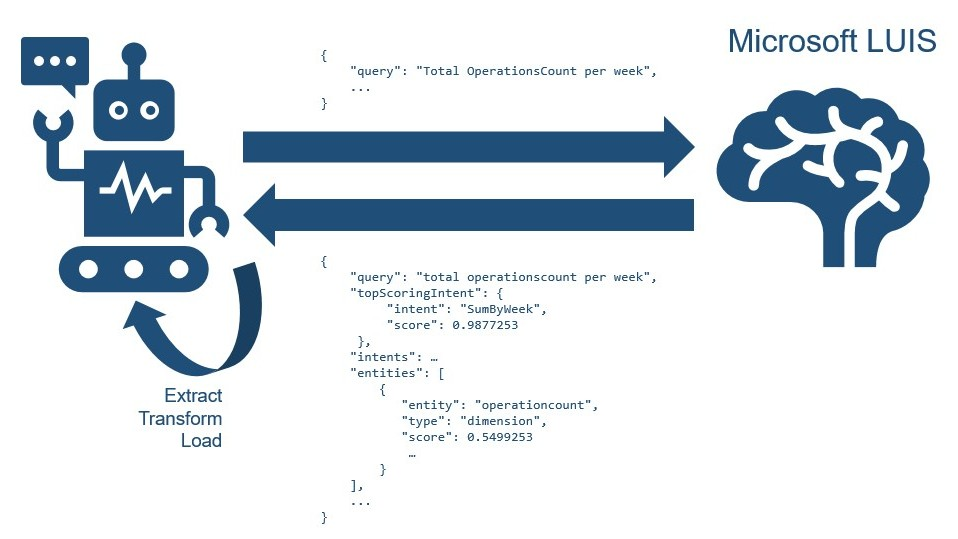
\includegraphics[width=.85\textwidth]{ch05/assets/prototype-implementation.jpg}
    \caption{Esquema referente à comunicação do \textit{chatbot} com o Microsoft LUIS}
    \label{fig:prototype_implementation}
\end{figure}

Os diagramas apresentados na Figura~\ref{fig:prototype_classworkflow} procuram detalhar a forma como foi desenhado o processo de extração de conhecimento. Ao receber uma mensagem, o \textit{Probot} recolhe o resultado devolvido pelo Microsoft LUIS e procura criar um novo \textit{Intent} de domínio aplicacional. Desta forma, usa-o para obter a resposta que deve apresentar. Por sua vez, o \textit{Intent} extrai a informação necessária do \textit{LuisResult}, gera a \textit{query} para comunicação com a fonte de dados (\textit{ProtoStore}) e finalmente, procura obter a informação necessária, gerando uma resposta adequada para o utilizador.  
%
\begin{figure}
\centering
    \begin{subfigure}{\textwidth}
        \centering
        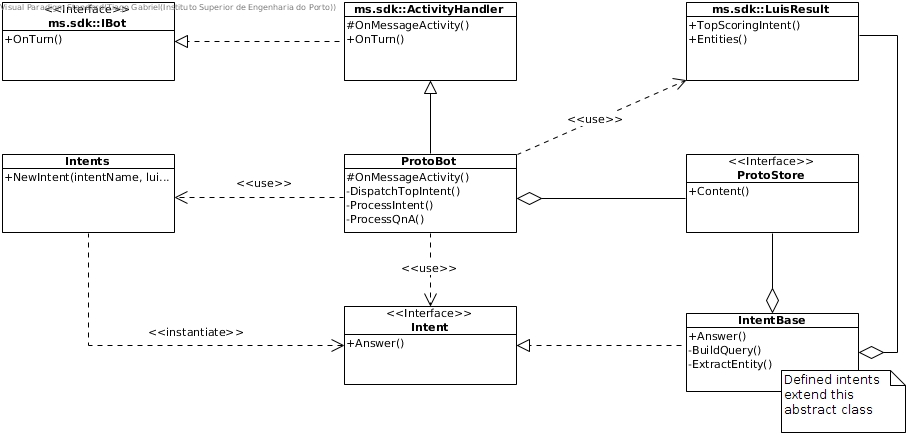
\includegraphics[width=.95\textwidth]{ch05/assets/prototype-classes.jpg}
        \caption{Vista genérica de classes usadas no protótipo}
     \end{subfigure}
     \bigbreak
     \bigbreak
     \begin{subfigure}{\textwidth}
         \centering
        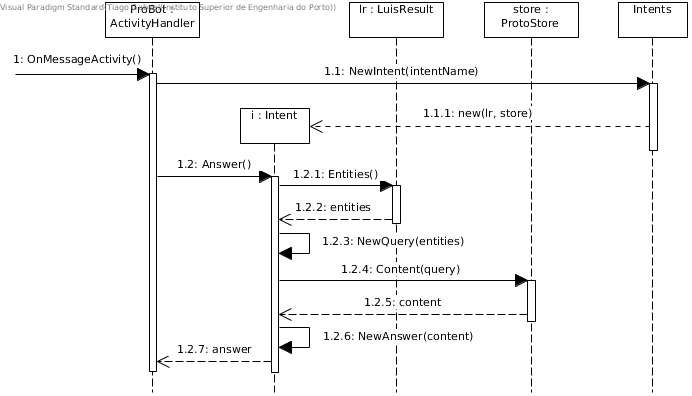
\includegraphics[width=\textwidth]{ch05/assets/prototype-workflow.jpg}
        \caption{Vista genérica do fluxo das classes usadas no protótipo}
     \end{subfigure}
\caption{Diagramas referentes à estrutura do protótipo na extração, transformação e carregamento da informação de domínio}
\label{fig:prototype_classworkflow}
\end{figure}

%%%%%%%%%%%%%%%%%%%%%%%%%%%%%%%%%
%           SECTION
%%%%%%%%%%%%%%%%%%%%%%%%%%%%%%%%%
\section{Síntese}
\label{sec:chap05_chaptersummary}
Neste capítulo abordaram-se os principais detalhes do protótipo \textit{Proto}, que foi desenvolvido de acordo com o modelo proposto. 

Inicialmente, expôs-se a sua especificação, tentando-se explicar a forma como o Microsoft LUIS e o QnA Maker seriam usados no contexto deste desenvolvimento e enquadrando a arquitetura do \textit{Proto} com a do modelo previamente idealizado.

Seguiu-se a interpelação ao processo de configuração das bases de conhecimento usando os serviços Microsoft, quer para respostas estáticas, quer para intenções e entidades. Relativamente a esta última, demonstraram-se aquelas que seriam esperadas para o protótipo, levando em consideração as perguntas definidas no âmbito dos critérios de sucesso (ver Secção~\ref{sec:chap01_solutionevaluation}).

No final, explicaram-se os conceitos particulares da implementação do \textit{Proto}, designadamente a forma como os metadados obtidos do Microsoft LUIS são extraídos, transformados e usados para o carregamento de informação da respetiva fonte de dados.